\documentclass[fleqn]{article}
\author{Authors from Deltares and USGS}

\usepackage{amsmath}
\usepackage{xcolor}
\usepackage{graphicx}
\graphicspath{{./figures/}}


\begin{document}

\title{Surface Water Flow in MODFLOW 6}
\maketitle

\tableofcontents

\section{Theoretical Development}
In this section ...

\subsection{Conservation of Mass}
Partial differential equation on conservation of mass:

\subsection{Manning's Equation}
Manning's equation is given as

\begin{equation}
  Q = \frac{1}{n} A R^{2 \over 3} \sqrt{S_f}
\end{equation}

\subsection{Storage Term}
The change in mass of water 

\subsection{Channel Cross Sections}

\section{Spatial Discretization}

\subsection{One-Dimensional Channel Network}

% This figure below is for the case where roughness varies for each line segment in the cross section 
\begin{figure}
	\centering
	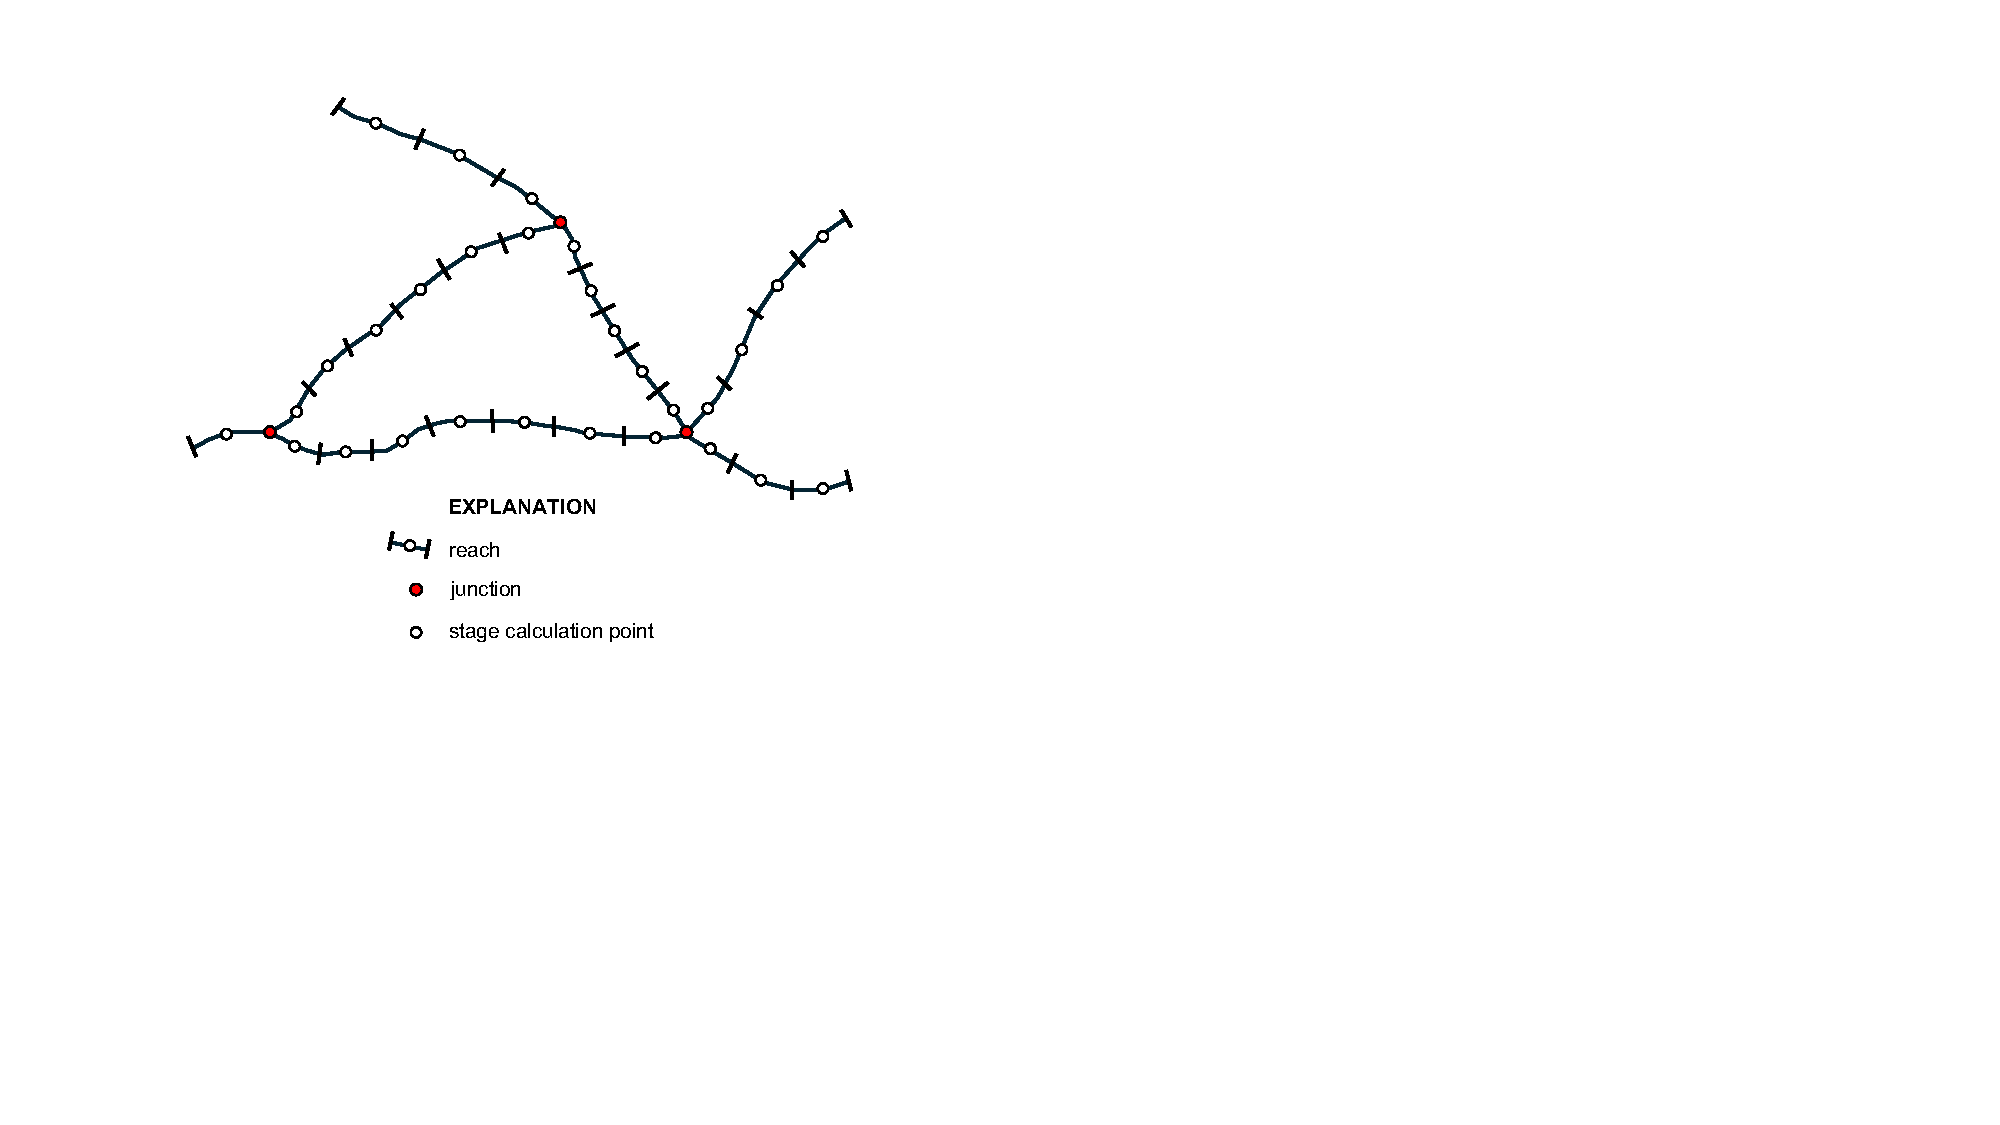
\includegraphics[scale=0.9]{figures/channel_network.pdf}
	\caption[Schematic showing a channel network.]{Schematic showing a channel network.  The channel network is discretized by the user into computational elements called reaches.  Stage is calculated within the reach at stage calculation points.  Stage calculations are typically located halfway between the reach start and reach end vertices, however, the user can adjust the fractional position of the stage calculation point along the reach.}
	\label{fig:channel_network}
\end{figure}

\subsection{Two-Dimensional Overland Flow}


\section{Numerical Solution}

\subsection{Newton-Raphson Method}

Flow throughout the connected channel network is based on a Newton-Raphson formulation, in which the following equation is formulated and solved simultaneously for each reach \textcolor{red}{change n and m to i and j?}

\begin{equation}
\label{eqn:nr-cvfd}
\begin{split}
\left ( \sum\limits_{m \in \eta_{n}} \frac{\partial Q_{n,m}}{\partial h_n} + \frac{\partial Q_{n,s}}{\partial h_n} - \frac{\partial Q_{STO}}{\partial h_n} \right ) h^k_n + 
\sum\limits_{m \in \eta_{n}} \frac{\partial Q_{n,m}}{\partial h_m} h^k_{m} = \\
- \left ( \sum\limits_{m \in \eta_{n}} Q_{n,m} + Q_{n,s} - Q_{STO} \right ) + \\
\left ( \sum\limits_{m \in \eta_{n}} \frac{\partial Q_{n,m}}{\partial h_n} + \frac{\partial Q_{n,s}}{\partial h_n} - \frac{\partial Q_{STO}}{\partial h_n} \right ) h^{k-1}_n + \sum\limits_{m \in \eta_{n}} \frac{\partial Q_{n,m}}{\partial h_m} h^{k-1}_{m}.
\end{split}
\end{equation}

\subsection{Discretized Flow Expression}

Manning's equation is written as

\begin{equation}
  Q = \frac{1}{n} A R^{2 \over 3} \sqrt{S_f}
\end{equation}

\noindent where $R$ is the hydraulic radius equal to $A / P$.  For the numerical implementation in MODFLOW we express Manning's equation as a product of a conductance term and the head difference between reach $n$ and $m$:

\begin{equation}
  Q_{nm} = C_{nm} \left ( h_m - h_n \right ).
\end{equation}

\noindent The conductance-based flow expression was selected so that individual conductances can be calculated for two connected reaches and then averaged together to give the conductance for the connection.  The average conductance between reach $n$ and reach $m$ ($C_{nm}$) is calculated by averaging a conductance for reach $n$ with a conductance for reach $m$.  The conductance for reach $n$, from the stage calculation point to the shared face with reach $m$, is denoted by $C_{n \rightarrow | m}$ and has dimensions of $L^2/T$.  The conductance for reach $m$, in the direction of reach $n$, is denoted by $C_{m \rightarrow | n}$ and also has dimensions of $L^2/T$.

The average conductance between reach $n$ and reach $m$ is calculated using the harmonic mean of $C_{n \rightarrow | m}$ and $C_{m \rightarrow | n}$ to give

\begin{equation}
  C_{nm} = \frac{C_{n \rightarrow | m}  C_{m \rightarrow | n}}{C_{n \rightarrow | m} + C_{m \rightarrow | n}}.
\end{equation}

\noindent The harmonic mean preferentially weights the average toward the lower of the two values and is based on piecewise constant reach properties that may change abruptly at the face between different reaches.

The conductance for reach $n$ in the $m$ direction ($C_{n \rightarrow | m}$) can be expressed as

\begin{equation}
  C_{n \rightarrow | m} = 
  \frac{
  A_n 
  R_{n}^{2 \over 3}
  }
  {n_n
  L_{n \rightarrow | m}
  \sqrt{| \gamma_n |}
  },
\label{eqn:cn}
\end{equation}


%\begin{equation}
%  C_{n \rightarrow | m} = 
% \frac{A_n R_{n}^{2 \over 3}}{n_n}
% \frac{1}{L_{n \rightarrow | m}}
% \frac{1}{ \sqrt{ \frac{ | \left ( h_m - h_n \right ) | } {L_{nm}}} }
%  \frac{1}{\sqrt{| \gamma_n |}}
%\end{equation}

%\begin{equation}
%  C_{n \rightarrow | m} = \frac{B_n}{ L_{nm} \sqrt{ \frac{ | \left ( h_m - h_n \right ) | } {L_{nm}}} }
%\end{equation}

\noindent where $A_n$ is the cross-sectional flow area ($L^2$) for reach $n$ calculated as a function of the water depth, $R_n$ is the hydraulic radius ($L$) for reach $n$, which is the cross-sectional flow area divided by the wetted perimeter, calculated as a function of the water depth, $n_n$ is the Manning's roughness coefficient ($T/L^{1 \over 3}$) for reach $n$,  $L_{n \rightarrow | m}$ is the distance ($L$) from the stage calculation point to the shared edge between reach $n$ and $m$, and $\gamma_n$ is the hydraulic gradient ($L^0$) for reach $n$.

Several of the terms in equation \ref{eqn:cn} are combined into a single term for reach $n$ called channel conveyance ($B_n$), which is defined as

\begin{equation}
  B_n = \frac{A_n R_n^{2 \over 3}}{n_n}.
\label{eqn:conveyance}
\end{equation}

\noindent Channel conveyance for reach $n$ is calculated as a function of an upstream-weighted water depth.  Thus, channel conveyance for reach $n$ can be written as

\begin{equation}
  B_n = \frac{A_n (d_u) R_n (d_u) ^{2 \over 3}}{n_n},
\label{eqn:conveyancedu}
\end{equation}

\noindent where the $A_n$ and $R_n$ terms include $(d_u)$ to indicate that they are calculated as a function of $d_u$.  $d_u$ is assigned to the depth of the reach (either $n$ or $m$) with the higher stage:

\[
d_u = 
\begin{cases}
  d_n & \text{if $h_n>h_m$} \\
  d_m & \text{otherwise}
\end{cases}.
\]

With this definition for channel conveyance, equation \ref{eqn:cn} can be simplified as

\begin{equation}
  C_{n \rightarrow | m} = 
  \frac{
  B_n 
  }
  {
  L_{n \rightarrow | m}
  \sqrt{| \gamma_n |}
  },
\label{eqn:cn}
\end{equation}

Channel conveyance is calculated in several different ways depending on how a cross section is defined for a reach.  For the cross sections shown in figure \ref{fig:cxs} a single Manning's roughness coefficient is assigned for the entire section.  If a single Manning's roughness coefficient is used to define the entire section for reach $n$, then the channel conveyance is calculated according to equation \ref{eqn:conveyance}.  If a cross section does not have a constant Manning's roughness coefficient for all line segments that define the channel, as shown for example in Figure \ref{fig:cxs_rough}, then a composite conveyance is calculated by summing the individual conveyance parts for the channel as

\begin{equation}
  B_n = \sum_{i=1}^{NLS} \frac{A_{n,i} \left ( \frac {A_{n,i}}{P_{n,i}}\right )^{2 \over 3}}{n_{n,i}},
\end{equation}

\noindent where $NLS$ is the number of line segments used to define the channel cross section.

% This figure below is for the case where roughness is the same for every line segment in the cross section 
\begin{figure}
	\centering
	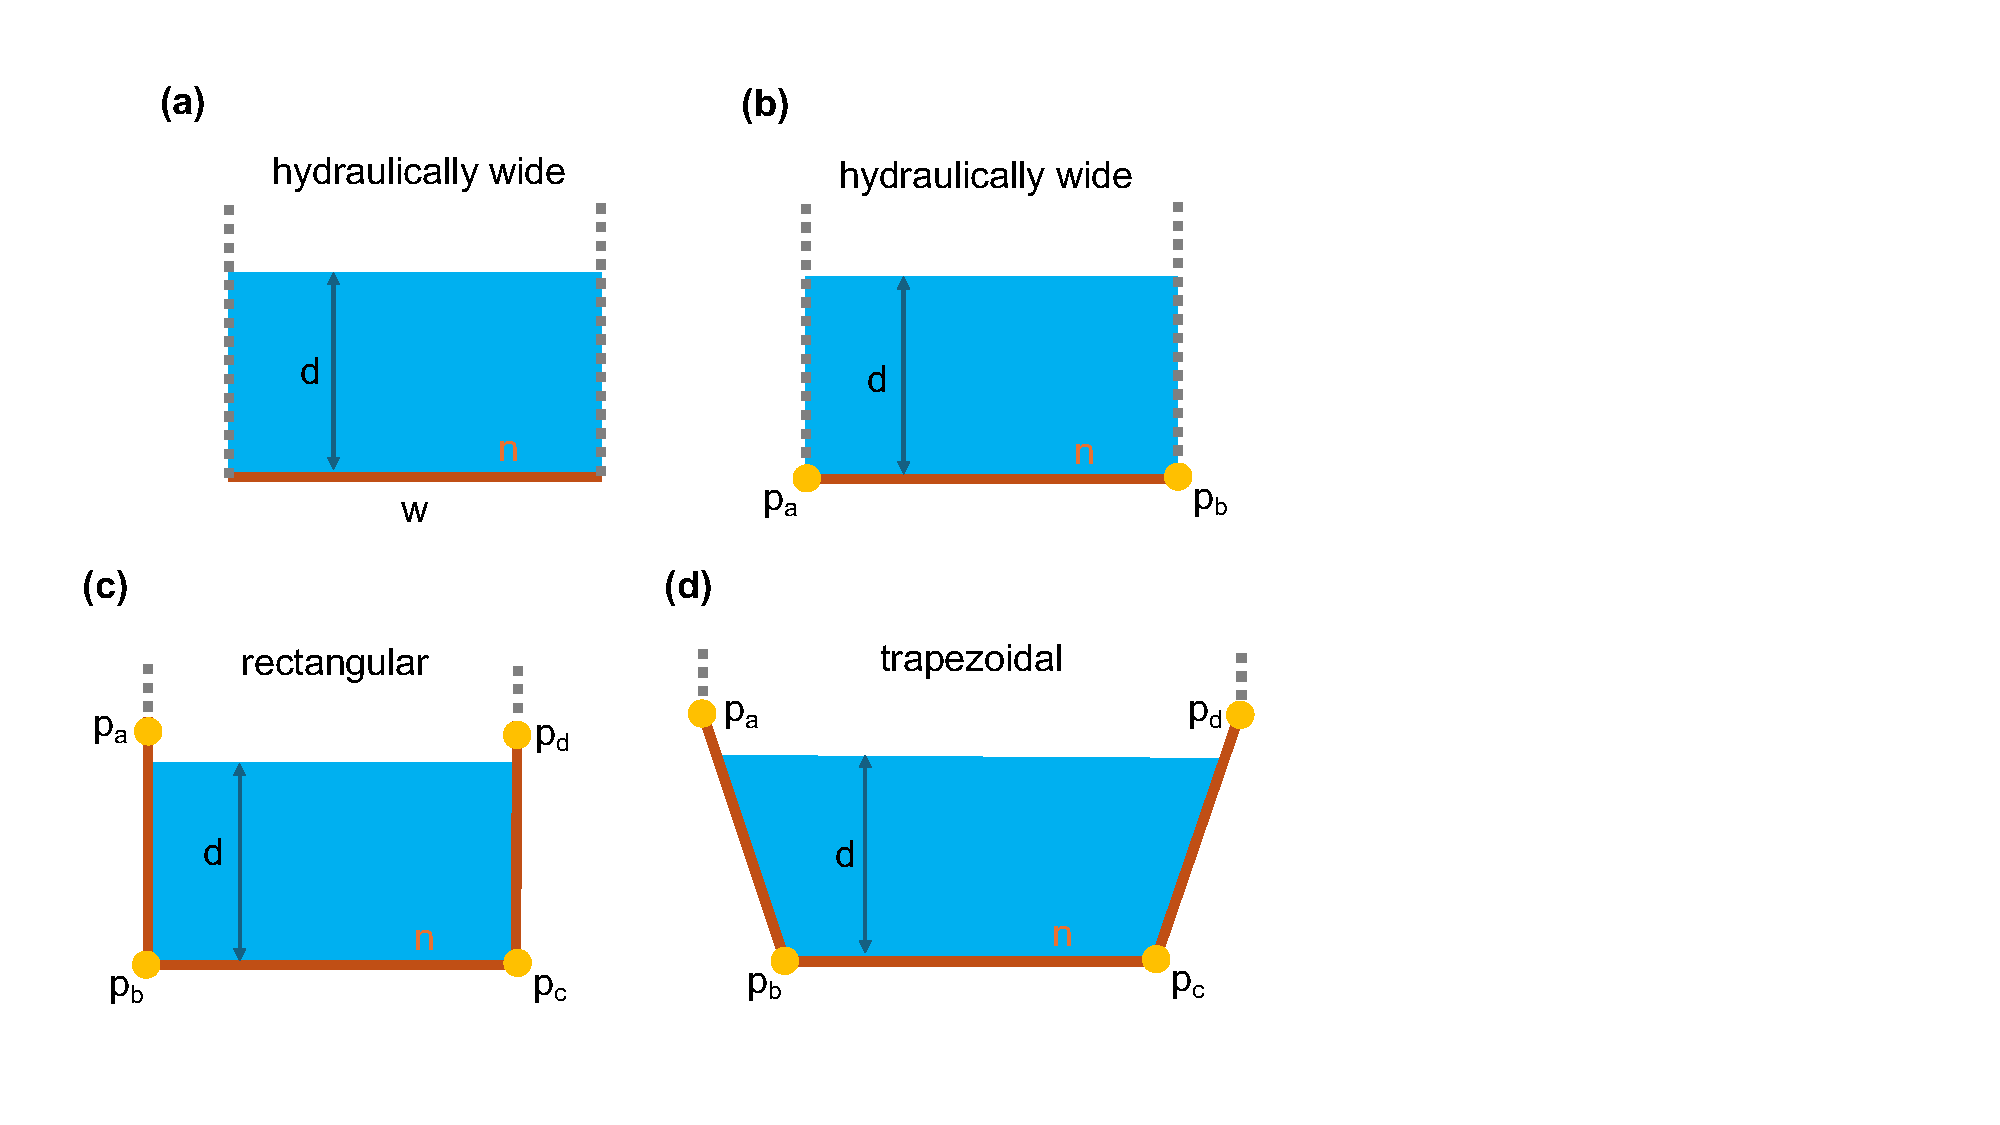
\includegraphics[scale=0.5]{figures/cxs.pdf}
	\caption[Schematic showing different types of channel cross sections with constant roughness.]{Schematic showing different types of cross sections with a single Manning's roughness coefficient $n$: (a) hydraulically wide cross section defined using the width input parameter; (b) hydraulically wide cross section defined using two points; (c) a rectangular cross section defined using four points, and (d) a trapezoidal cross section defined using four points.  For the hydraulically wide rectangular cross sections in (a) and (b) the model does not include any channel resistance for the vertical wetted sections corresponding to the dashed lines.  For cross sections shown in (c) and (d), if the water surface rises above the channel points, no channel resistance is included for sections above the uppermost points}
	\label{fig:cxs}
\end{figure}

% This figure below is for the case where roughness varies for each line segment in the cross section 
\begin{figure}
	\centering
	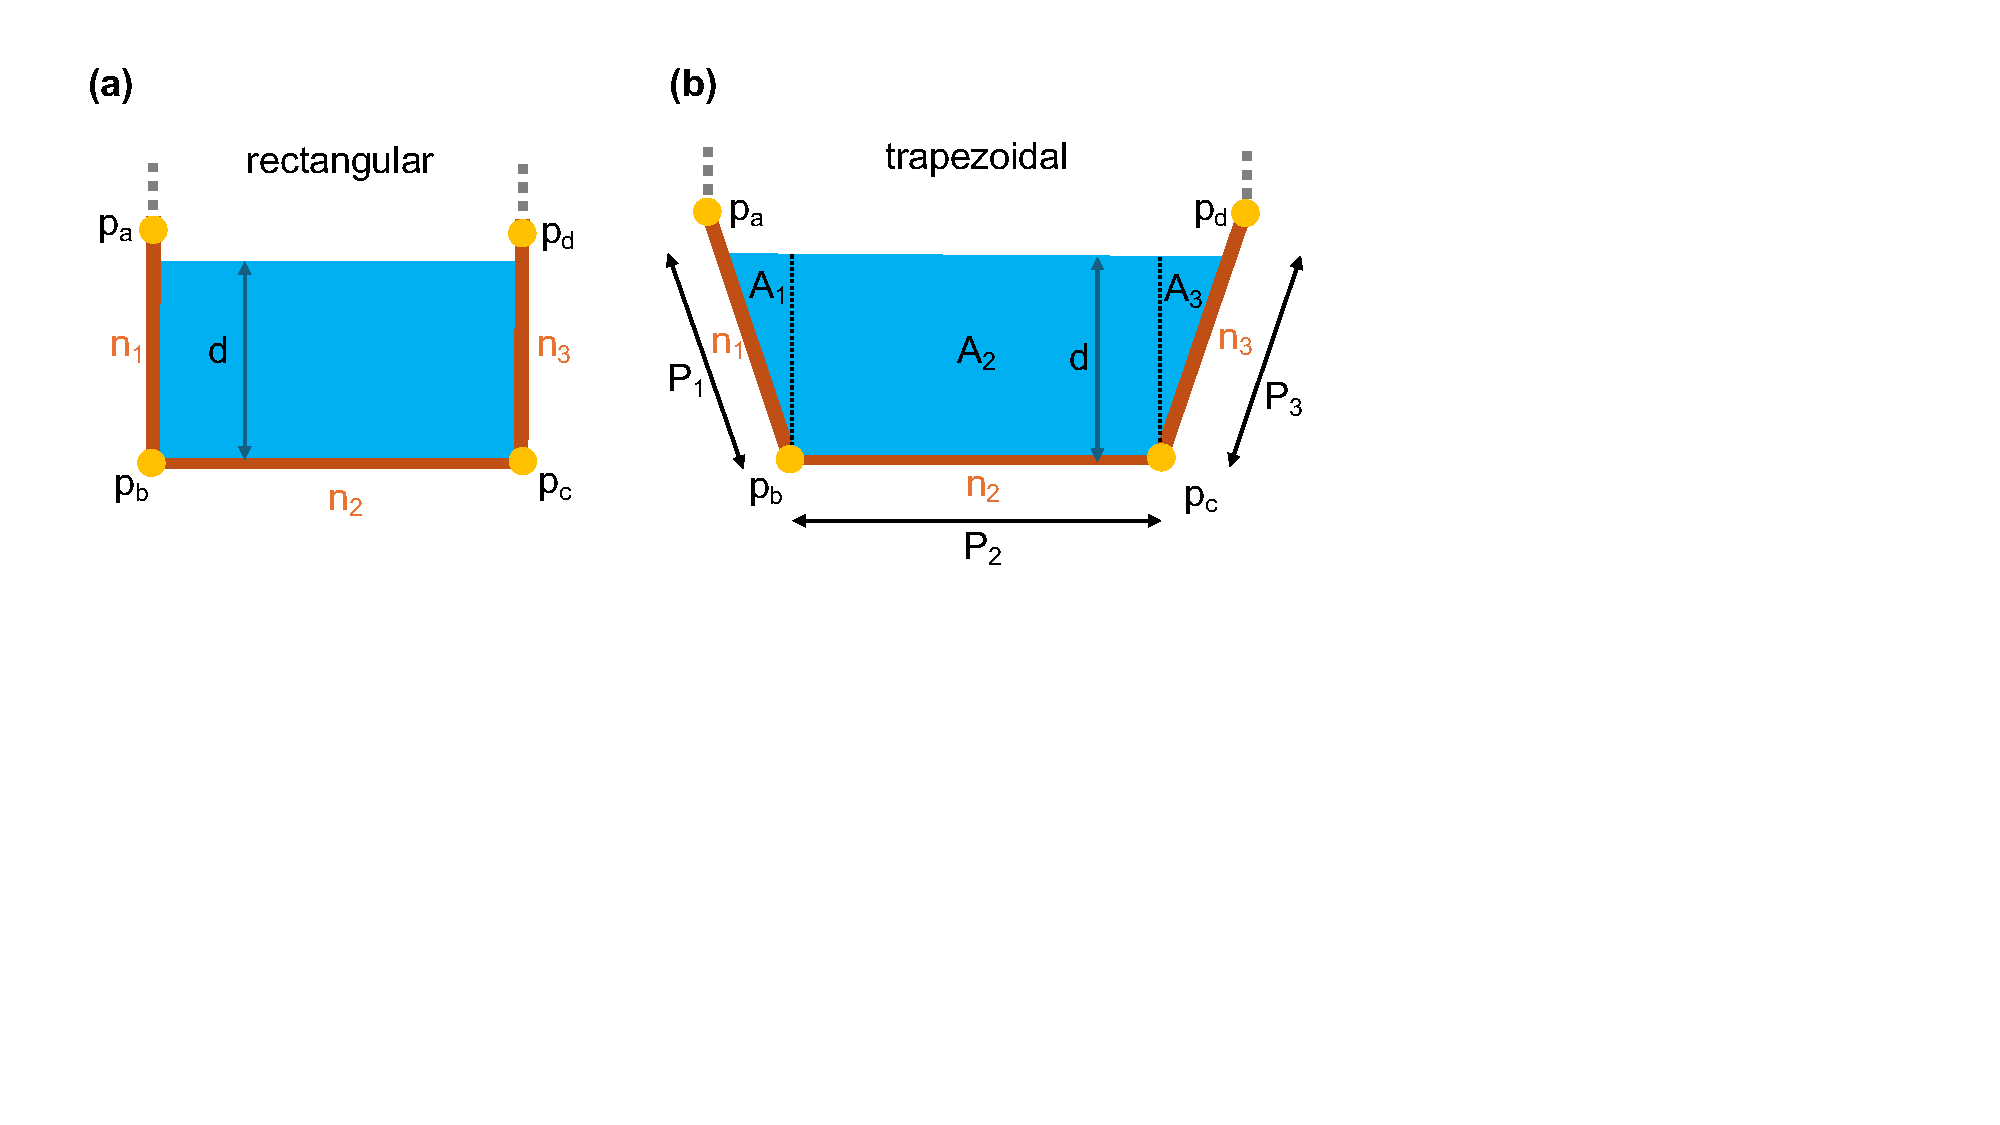
\includegraphics[scale=0.5]{figures/cxs_rough.pdf}
	\caption[Schematic showing different types of channel cross sections with variable roughness.]{Schematic showing different types of cross sections with variable Manning's roughness coefficient: (a) a rectangular cross section defined using four points, and (b) a trapezoidal cross section defined using four points.  The Manning's roughness coefficient is varies by line segment.  If the water surface rises above the channel points, no channel resistance is included for sections above the uppermost points}
	\label{fig:cxs_rough}
\end{figure}


\subsection{Temporal Discretization}
Adaptive time stepping

\subsection{Sources and Sinks}

\subsection{Initial and Boundary Conditions}

A zero-depth-gradient (ZDG) boundary condition can be assigned to any reach to allow from the channel.  Flow out of the channel is calculated as

\begin{equation}
  Q = \frac{1}{n}A R^{2/3} \sqrt{S_0}
\end{equation}


\section{Integration into MODFLOW 6}

\section{Examples}

\subsection{Tilted V-Catchment}

Example problem is described by \cite{digiammarco1996}, \cite{VanderKwaak1999}, and \cite{panday2004}.

\begin{figure}
	\centering
	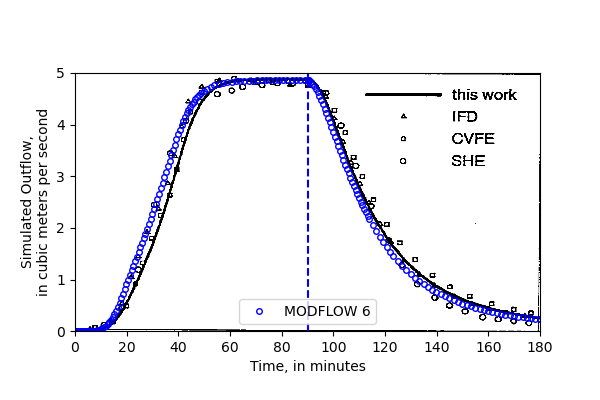
\includegraphics[scale=1.]{figures/vcatch.png}
	\caption[Simulated outflow for the tilted v-catchment example.]{Simulated outflow for the tilted v-catchment example.  MODFLOW 6 results are shown on top of Figure 4-10a in \cite{VanderKwaak1999}.  Dashed blue line separates the first 90-minute period with rainfall from the second 90-minute period with no rainfall.}
	\label{fig:vcatch}
\end{figure}

\bibliographystyle{plain}
\bibliography{swfref} 

\end{document}